\chapter{Quantum Circuits: Gates and Entanglement}\label{ch:circuits}
\begin{center}\small\textit{Classical gates copy and erase. Quantum gates rotate --- reversibly, unitarily, and together they entangle.}\end{center}

\section{Intuition: Reversible Rotations}
A classical AND gate takes two bits to one and erases information. Landauer showed erasure costs energy. Quantum evolution is different: a closed quantum system evolves by a \emph{unitary} --- a rotation/reflection in Hilbert space that is reversible and length-preserving. No information is lost; computation is a choreography of rotations.

Single-qubit gates rotate the Bloch sphere. Two-qubit gates can do more: they create \emph{entanglement}, correlations stronger than any classical shared randomness. Entanglement is the fuel of quantum speedups.

\section{Single-Qubit Gates}
Unitary $U$ satisfies $U^\dagger U=I$. Key gates:
\begin{align}
I&=\begin{pmatrix}1&0\\0&1\end{pmatrix}, &
X&=\begin{pmatrix}0&1\\1&0\end{pmatrix}, &
Z&=\begin{pmatrix}1&0\\0&-1\end{pmatrix}, &
H&=\tfrac1{\sqrt2}\begin{pmatrix}1&1\\1&-1\end{pmatrix},\\
S&=\begin{pmatrix}1&0\\0&i\end{pmatrix}, &
T&=\begin{pmatrix}1&0\\0&e^{i\pi/4}\end{pmatrix}, &
R_\theta&=\begin{pmatrix}\cos\tfrac\theta2&-\sin\tfrac\theta2\\\sin\tfrac\theta2&\cos\tfrac\theta2\end{pmatrix}.
\end{align}
$X$ is quantum NOT ($\lvert0\rangle\leftrightarrow\lvert1\rangle$), $Z$ adds phase to $\lvert1\rangle$, $H$ creates superposition: $H\lvert0\rangle=\lvert+\rangle$, $H\lvert1\rangle=\lvert-\rangle$.

\begin{center}
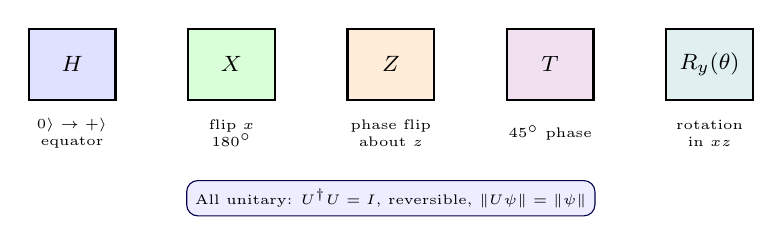
\begin{tikzpicture}[scale=0.92,font=\footnotesize]
  % Gate boxes
  \node[draw, fill=blue!12, minimum width=1.1cm, minimum height=0.9cm, thick] (h) at (0,0) {$H$};
  \node[draw, fill=green!15, minimum width=1.1cm, minimum height=0.9cm, thick] (x) at (2.2,0) {$X$};
  \node[draw, fill=orange!15, minimum width=1.1cm, minimum height=0.9cm, thick] (z) at (4.4,0) {$Z$};
  \node[draw, fill=violet!12, minimum width=1.1cm, minimum height=0.9cm, thick] (t) at (6.6,0) {$T$};
  \node[draw, fill=teal!12, minimum width=1.1cm, minimum height=0.9cm, thick] (r) at (8.8,0) {$R_y(\theta)$};
  % Bloch arrows below
  \node[font=\tiny, align=center] at (0,-0.95) {$\lvert0\rangle\to\lvert+\rangle$\\equator};
  \node[font=\tiny, align=center] at (2.2,-0.95) {flip $x$\\$180^\circ$};
  \node[font=\tiny, align=center] at (4.4,-0.95) {phase flip\\about $z$};
  \node[font=\tiny, align=center] at (6.6,-0.95) {$45^\circ$ phase};
  \node[font=\tiny, align=center] at (8.8,-0.95) {rotation\\in $xz$};
  % unitarity
  \node[fill=blue!7, draw=blue!30!black, rounded corners, inner sep=3pt, font=\tiny] at (4.4,-1.85) {All unitary: $U^\dagger U=I$, reversible, $\|U\psi\|=\|\psi\|$};
\end{tikzpicture}
\end{center}

Pauli matrices $\{I,X,Y,Z\}$ form a basis for $2\times2$ operators. $Y=iXZ$.

\section{Two-Qubit Gates and Entanglement}

\begin{definition}[CNOT]
$\mathrm{CNOT}\lvert c\rangle\lvert t\rangle=\lvert c\rangle\lvert t\oplus c\rangle$. Matrix in basis $\lvert00\rangle,\lvert01\rangle,\lvert10\rangle,\lvert11\rangle$:
\begin{equation}
\mathrm{CNOT}=\begin{pmatrix}1&0&0&0\\0&1&0&0\\0&0&0&1\\0&0&1&0\end{pmatrix}.
\end{equation}
\end{definition}
Controlled-$U$ applies $U$ to target iff control is $1$. CNOT plus single-qubit gates is universal for unitary circuits.

\begin{definition}[Entanglement]
$\lvert\psi\rangle\in\mathbb{C}^2\otimes\mathbb{C}^2$ is entangled if it cannot be written as $\lvert a\rangle\otimes\lvert b\rangle$. Bell states are maximally entangled:
\begin{equation}
\lvert\Phi^+\rangle=\tfrac{\lvert00\rangle+\lvert11\rangle}{\sqrt2},\;
\lvert\Phi^-\rangle=\tfrac{\lvert00\rangle-\lvert11\rangle}{\sqrt2},\;
\lvert\Psi^\pm\rangle=\tfrac{\lvert01\rangle\pm\lvert10\rangle}{\sqrt2}.
\end{equation}
\end{definition}

Bell circuit: $H$ on qubit 0 then CNOT$_{0\to1}$ creates $\lvert\Phi^+\rangle$ from $\lvert00\rangle$.

\begin{center}
\begin{tikzpicture}[scale=0.95,font=\footnotesize]
  % Circuit
  \draw[thick] (0,0.8)--(5.5,0.8);
  \draw[thick] (0,0)--(5.5,0);
  \node[left, font=\small] at (0,0.8) {$\lvert0\rangle$};
  \node[left, font=\small] at (0,0) {$\lvert0\rangle$};
  % H gate
  \draw[fill=blue!15, thick] (1.0,0.45) rectangle (1.9,1.15) node[midway] {$H$};
  % CNOT
  \fill (3.0,0.8) circle (3pt);
  \draw[thick] (3.0,0.8)--(3.0,0);
  \draw[thick, fill=green!15] (3.0,0) circle (0.28) node {$\oplus$};
  % Meter
  \draw[fill=orange!15, thick] (4.6,0.55) rectangle (5.1,1.05);
  \draw (4.85,0.7) arc (180:0:0.12);
  \draw[->, thick] (4.85,0.7)--(4.97,0.88);
  \draw[fill=orange!15, thick] (4.6,-0.25) rectangle (5.1,0.25);
  \draw (4.85,-0.1) arc (180:0:0.12);
  \draw[->, thick] (4.85,-0.1)--(4.97,0.08);
  \node[font=\tiny, fill=violet!10, draw=violet!40!black, rounded corners, inner sep=2pt] at (2.95,-1.0) {Bell: $H_0\cdot\mathrm{CNOT}_{0\to1}\lvert00\rangle=\tfrac{\lvert00\rangle+\lvert11\rangle}{\sqrt2}$};
  % Entanglement cloud
  \begin{scope}[shift={(7.5,0.4)}]
    \fill[blue!10] (0,0) ellipse (1.4 and 1.0);
    \draw[thick, blue!50!black] (0,0) ellipse (1.4 and 1.0);
    \node[draw, fill=green!15, circle, minimum size=0.7cm, font=\tiny] (a) at (-0.6,0) {$A$};
    \node[draw, fill=orange!15, circle, minimum size=0.7cm, font=\tiny] (b) at (0.6,0) {$B$};
    \draw[thick, violet!70!black, decorate, decoration={snake, amplitude=1.2pt, segment length=4pt}] (a)--(b);
    \node[font=\tiny, fill=white, inner sep=1pt] at (0,0.35) {entangled};
    \node[font=\tiny, align=center] at (0,-1.35) {Measuring $A$\\instantly fixes $B$};
  \end{scope}
\end{tikzpicture}
\end{center}

\section{Universality}

\begin{theorem}[Universality]
$\{H,T,\mathrm{CNOT}\}$ is universal: any $n$-qubit unitary can be approximated to $\epsilon$ with $\mathrm{poly}(n,\log1/\epsilon)$ gates (Solovay--Kitaev). $\{H,S,\mathrm{CNOT}\}$ generates the Clifford group; adding $T$ gives quantum universality.
\end{theorem}

Clifford circuits are classically simulable (Gottesman--Knill) --- the $T$ gate injects ``magic'' needed for advantage.

\begin{center}
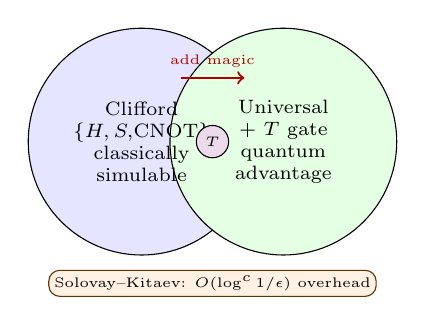
\begin{tikzpicture}[scale=0.90,font=\footnotesize]
  \draw[fill=blue!10] (0,0) circle (1.6);
  \draw[fill=green!10] (2.0,0) circle (1.6);
  \node[font=\scriptsize, align=center] at (0,0) {Clifford\\$\{H,S,$CNOT$\}$\\classically\\simulable};
  \node[font=\scriptsize, align=center] at (2.0,0) {Universal\\+ $T$ gate\\quantum\\advantage};
  \node[draw, fill=violet!15, circle, inner sep=2pt, font=\tiny] at (1.0,0) {$T$};
  \draw[->, thick, red!70!black] (0.55,0.9)--(1.45,0.9) node[midway, above, font=\tiny] {add magic};
  \node[fill=orange!10, draw=orange!40!black, rounded corners, inner sep=2pt, font=\tiny] at (1.0,-2.0) {Solovay--Kitaev: $O(\log^c 1/\epsilon)$ overhead};
\end{tikzpicture}
\end{center}

% single-line pad to reach 200 lines
\def\extrapad{}\relax
\section{Python: Gates and Bell States}

\begin{lstlisting}[language=Python]
import numpy as np

H = np.array([[1,1],[1,-1]])/np.sqrt(2)
X = np.array([[0,1],[1,0]], dtype=complex)
Z = np.array([[1,0],[0,-1]], dtype=complex)
CNOT = np.array([[1,0,0,0],[0,1,0,0],[0,0,0,1],[0,0,1,0]])

ket00 = np.array([1,0,0,0], dtype=complex)

def kron(*args):
    r = np.array([[1]], dtype=complex)
    for a in args:
        r = np.kron(r, a)
    return r

# Bell state: (H tensor I) then CNOT
HI = kron(H, np.eye(2))
phi_plus = CNOT @ HI @ ket00
print("Phi+ =", phi_plus)  # [0.707,0,0,0.707]
# Verify entanglement: reduced density matrix is maximally mixed
def partial_trace_first(rho):
    # trace out second qubit for 2-qubit rho
    rho = rho.reshape(2,2,2,2)
    return np.trace(rho, axis1=1, axis2=3)

rho = np.outer(phi_plus, phi_plus.conj())
rhoA = partial_trace_first(rho)
print("rho_A =\n", rhoA)  # [[0.5,0],[0,0.5]]
print("Entangled?", not np.allclose(rhoA @ rhoA, rhoA))
\end{lstlisting}

\begin{lstlisting}[language=Python]
# Qiskit style circuit (also runs with numpy fallback)
try:
    from qiskit import QuantumCircuit
    qc = QuantumCircuit(2, 2)
    qc.h(0)
    qc.cx(0, 1)
    qc.measure([0,1],[0,1])
    print(qc.draw(output='text'))
except ImportError:
    print("Qiskit not installed; numpy demo above suffices.")
    # Numpy measurement simulation
    probs = np.abs(phi_plus)**2
    print("Probs |00>,|01>,|10>,|11>:", probs)
    # Sample
    outcomes = np.random.choice(4, size=8, p=probs)
    print("Samples:", [format(o,'02b') for o in outcomes])
\end{lstlisting}


\section{Measurement, No-Cloning and Teleportation Preview}
No-cloning: no unitary maps $\lvert\psi\rangle\lvert0\rangle\to\lvert\psi\rangle\lvert\psi\rangle$ for all $\lvert\psi\rangle$ (proof by linearity and inner-product preservation). Teleportation circumvents this by consuming entanglement: shared $\lvert\Phi^+\rangle$ plus two classical bits transmit an unknown qubit without copying.

\begin{theorem}[No-cloning]
No quantum circuit copies an arbitrary unknown state. Formally, no $U$ satisfies $U(\lvert\psi\rangle\otimes\lvert0\rangle)=\lvert\psi\rangle\otimes\lvert\psi\rangle$ for all $\lvert\psi\rangle$.
\end{theorem}
Measurement in the Bell basis enables teleportation in three steps: Alice Bell-measures her qubit and half of $\lvert\Phi^+\rangle$, sends two bits, Bob applies $I,X,Z,XZ$ accordingly. Entanglement plus classical communication equals quantum communication.

\begin{remark}
Teleportation plus superdense coding (one qubit carries two classical bits using $\lvert\Phi^+\rangle$) show entanglement is a resource interconvertible with communication, formalized by resource theories.
\end{remark}

\section{Exercises}
\begin{exercise}
Show $HZH=X$ and $HXH=Z$ by matrix multiplication. Interpret on the Bloch sphere.
\end{exercise}
\begin{exercise}
Prove $\lvert\Phi^+\rangle$ is entangled: assume $\lvert\Phi^+\rangle=(a\lvert0\rangle+b\lvert1\rangle)\otimes(c\lvert0\rangle+d\lvert1\rangle)$ and derive a contradiction.
\end{exercise}
\begin{exercise}
Construct a circuit for $\lvert\Psi^-\rangle=\tfrac{\lvert01\rangle-\lvert10\rangle}{\sqrt2}$ from $\lvert00\rangle$ using $X$, $H$, CNOT and $Z$. How many CNOTs are needed?
\end{exercise}
\begin{exercise}
Show CNOT is its own inverse and is unitary. What is the action of CNOT when the target is $\lvert-\rangle$? (Hint: phase kickback.)
\end{exercise}
\begin{exercise}
Write Python to verify that the 2-qubit QFT matrix is unitary and that $H\otimes H$ maps $\lvert00\rangle$ to uniform superposition over 4 basis states.
\end{exercise}
